%srj
%aum gaanathipathaye namaha
 %aum gaanathipathaye namaha
%srj


\section{Scalable Function Matching}\label{sec:func_match}
%This section, we present the four modules in \tool in details.
%As the first step, \tool disassembles the binary and splits it into basic functional units or functions. Then, it constructs the control-flow graph (CFG) for each function, where each CFG is consists of basic-blocks. Later, the constructed CFGs are used to generate the partial traces.

%\subsection{Partial Trace Extraction} \label{subsec:partial_trace}

In \tool and \toolNew, similarity matching is done at the granularity of function and sub-function levels (i.e., we can match a part of a target function to the signature function).




\subsection{Primary Matching} \label{subsec:matching:primary}
In primary matching, high-level semantic features and structural features are combined to measure the semantic similarity of the two code segments as the granularity of function. Let $\mathcal{SIM_{H}}(sig, tar)$  denote the similarity score of using high-level semantic features and $\mathcal{SIM_{S}}(sig, tar)$ denote the similarity score of using structural features.
The former score is measured by Jaccard containment similarity~\cite{agrawal2010indexing}, considering each function has a bag of high-level semantic features:
\begin{equation}
\begin{aligned}
\mathcal{SIM_{H}}(sig, tar) = \frac{\mathcal{H}_{sig} \bigcap \mathcal{H}_{tar}}{\mathcal{H}_{sig}}
\end{aligned}
\end{equation}

\xyx{Specifically, for each of six types of high-level semantic features, the Jaccard distance is calculated, and the overall $\mathcal{SIM_{H}}(sig, tar)$  is the mean value of Jaccard distances of different types of high-level semantic features. Note that if both signature function and target function have no function calls, then features in terms of function call tags, function call sequence, function parameters are not available, and they are not counted in overall similarity.}

The latter score is measured by calculating FDD (Definition 3 in \S\ref{sec:category:structralFea}), and the FDD value is already normalized into  the range between 0 to 1. $\mathcal{SIM_{S}}(sig, tar)$ is to convert the distance to the similarity:
\begin{equation}
\begin{aligned}
 \mathcal{SIM_{S}}(sig, tar) = Convert(FDD(sig, tar)) \\
 = 1 - FDD(sig, tar)%\frac{FDD(sig, tar)}{w'_{sig} + w'_{tar}}
\end{aligned}
\end{equation}
%\begin{equation}
%\begin{aligned}
% Norm(FDD(sig, tar))
%\end{aligned}
%\end{equation}
%where $w'_{sig}$ and $w'_{tar}$ denote the number of weighted assembly instructions in function $sig$ and function $tar$, respectively.
The idea of convertion is that if these two functions' distance is closer to 0, their similarity is closer to 1. Vice versa, if their distance is as big as it could possibly be, their similarity is prone to be 0.

Once we have similarity scores in high-level semantics and structures, the primary matching result $\mathcal{SIM^\prime}(sig, tar)$ is calculated as the weighted sum of $\mathcal{SIM_{H}}(sig, tar)$ and $\mathcal{SIM_{S}}(sig, tar)$, which is defined as follow:
\begin{equation}
\begin{aligned}
 \mathcal{SIM^\prime}(sig, tar) =  (1 - \mathcal{W}/2) *  \mathcal{SIM_{H}}(sig, tar)  \\
  + ( \mathcal{W}/2) * \mathcal{SIM_{S}}(sig, tar)
\end{aligned}
\end{equation}
where $\mathcal{W}$ = $min(\frac{w'_{sig}}{ w'_{tar}}, \frac{w'_{tar}}{ w'_{sig}})$ and $\mathcal{W}$ means the ratio of these two functions' instruction number.

Hence, the idea of primary matching is straightforward --- structural features are effective when the sizes of two functions are similar. If two functions have the similar size of instructions, structural features have the same weight as high-level semantic features. If not, high-level semantic features have more weight than structural features. According to this idea, a high value of $\mathcal{SIM^\prime}(sig, tar)$ (e.g., $\geq 0.8$) indicates that $sig$ and $tar$ are similar in both structures and high-level semantics.

\subsection{Low-level Semantic Features Matching} \label{subsec:matching:lowFea}
%\footnote{Signature function refers to the search query function in hand, whereas target functions refer to functions in the target binary pool against which the signature function is matched.}
When the primary matching does not find any ranked results that are of high $\mathcal{SIM^\prime}(sig, tar)$ values, low-level semantic features are used.
Note that low-level semantics refer to not only the implementation details, but also the partial semantics of the function.
To this end, we propose the function model consisting of partial traces of various lengths, %, a variant of tracelet~\cite{DBLP:conf/pldi/DavidY14},
which is more flexible in terms of comparison granularity, compared with the BB-centric
%and tracelet~\cite{DBLP:conf/pldi/DavidY14} based
function modelling~\cite{DBLP:conf/sp/PewnyGGRH15,luo2014semantics}. Then, from these partial traces we extract symbolic expressions. Based on I/O values for register, flags and memory addresses, we match the partial traces inside two functions. %To reduce the noise, we remove the partial traces that are infeasible to reach (via solving the symbolic expressions) or are specific to compilers.
Last, we apply Jaccard containment similarity~\cite{agrawal2010indexing} to measure the similarity score of two function models.
%That is, for each function, we generate partial traces of various lengths (called, \textit{k-length partial traces}), where by varying the length, the semantics of the function is captured at various granularity levels.
%granularity of single building block is adjusted\footnote{Length of one yields a basic-block centric models, where the basic-block is considered as a single building block.}.
\subsubsection{K-length Partial Trace Extraction} \label{subsec:partial_trace_ext}
Our partial trace extraction is based on the technique proposed by David \emph{et. al.}~\cite{DBLP:conf/pldi/DavidY14}.
We omit the algorithm and explain the results using one example.
Fig.~\ref{fig:example-cfg} depicts a sample CFG of a function and the extracted 2- and 3-length partial traces (i.e., for $k=2,3$). We can observe that the original control-flow instructions (\texttt{jnb}, and \texttt{jb}) are omitted as the flow of execution is already determined. Note that the feasibility of the flow of executions is not considered at this step. %In \S\ref{subsubsec:sou_prun}, we show how the partial traces which are \textit{infeasible} to reach are identified via constraint solving and removed. %from our analysis. Here, infeasible partial traces refer to program execution flows that are not possible to reach during any concrete execution.

\begin{figure}[]
\begin{center}\vspace{-3mm}
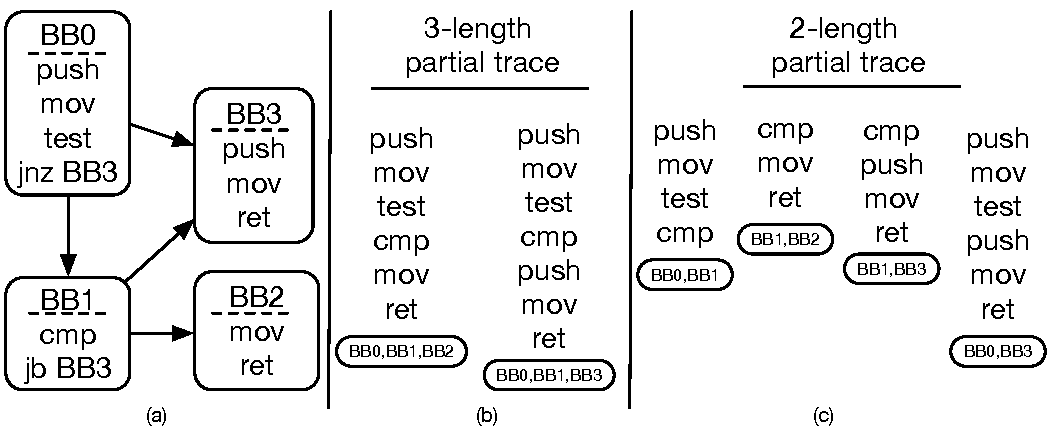
\includegraphics[width=7.5cm]{srj-figures/srj-partial_trace_ex.pdf} %\vspace{-1mm}
\caption{A sample CFG (a) and the extracted 3-length (b) and 2-length (c) partial traces}
\label{fig:example-cfg} \vspace{-2mm}
\end{center}
\end{figure}
%
%\subsection{Trace Pruning}\label{subsec:trace_prun}
%In \tool, we adopt two trace pruning methods to reduce the noise in the results and also to speed up the matching process.
%%steps to reduce the noise in I/O samples based function \textit{similarity} matching, which is less precise than the unscalable function \textit{equivalence} matching.}
%\subsubsection{Infeasible Partial Trace Pruning} \label{subsubsec:sou_prun}
%\tool is a static analysis based tool, and therefore it is difficult (or even impossible) to identify all the infeasible partial traces in practice. In \tool, we prune the obviously infeasible partial traces via the constraint solver. Given the symbolic expressions extracted from a partial trace, we rely on the constraint solver to determine whether all the constraints present in the symbolic expressions can be satisfied. %If not, that relevant partial trace is considered infeasible.
%As we use the constraint solver to generate I/O samples in \S\ref{subsec:sem_fea_ext}, we need no additional effort to identify the infeasible partial traces --- if the constraint solver is unable to find appropriate concrete values for the pre- and post-state variables, the relevant partial trace is considered infeasible.
%%That is, given a partial trace, we extract the set of I/O formulas, as explained in Section~\ref{subsec:stat_sem}, and try to generate a model that satisfied all the constraints present in the I/O formulas (i.e., able to generate appropriate concrete values for input/out vocabularies), if such model is not available then that partial trace is considered infeasible.
%%and pass them to the solver, which will try to solve the constraints and generate a model that satisfies them all. If the solver fails to generate a model, we label that partial trace as infeasible and prune it from the analysis.
%
%We also observe that some  partial traces, for which the solver is able to generate models (or I/O samples), might be infeasible during actual execution, as the feasibility of their paths depends on various factors, such as global variables, values in the heap and other dynamic data, that are beyond the scope of our analysis. Further, in general, infeasible path elimination (or detection) by itself is a hard problem~\cite{bodik1997refining}. However, compared with the static analysis solutions proposed in the literature~\cite{DBLP:conf/pldi/DavidY14,pewny2014leveraging,DBLP:conf/sp/PewnyGGRH15}, this work makes an attempt to reduce the search candidates using a pruning technique.
%
%%Even with the infeasible partial traces pruned, it is still difficult to compare the signature function against those functions in the target binary pool. Thus, a systematic way of performing the similarity matching among partial traces is desired. Specifically, the question ``what length of partial traces in the search query needs to be matched with what length of partial traces in the target function?'' still persists.
%
%
%
%
%\subsubsection{Compiler Specific Code Pruning}
%%%Compiler idioms capture the compilation information, via code patterns  commonly  included for a specific compilation option during compilation process.
%%%\noindent \textbf{Compiler idiom}
%%%These idioms help to identify the additional code included by the compiler during compilation process.
%Based on the compilation option selected, the compiler could include additional code (i.e., code that is not originally written by the programmer) into the compiled binary. For example, there are more than 150 compiler options available for both \texttt{gcc} and \texttt{MS Visual Studio}, which a programmer can choose from when compiling her program. Some of these options result in adding extra code into the binary (e.g., \texttt{stack-smashing protection} or SSP shown in Fig.~\ref{fig:gcc_ssp}). The code segments in the function prologue and epilogue in Fig.~\ref{fig:gcc_ssp} ensure the stack integrity is not violated. These code segments are automatically included by the \texttt{gcc} compiler when the option for stack smash protection is enabled.
%%(using either \texttt{-fstack-protector-all} or \texttt{-fstack-protector} flag).
%%(using either -$\mathtt{fstack}$-$\mathtt{protector}$-$\mathtt{all}$ or -$\mathtt{fstack}$-$\mathtt{protector}$ flag).
%
%In similarity matching between the signature and target functions, the additional compiler specific code can introduce noise by changing the code structures and diluting the similar parts, especially when the functions are small.
% %the additional code included by the compiler might influence the similarity score between the signature and target functions, especially when the functions are relatively small.
%% Therefore, in order to avoid imprecise similarity matching, the compiler specific code need to be removed from the partial traces.
%Thus, it is necessary to identify and remove the compiler specific code from the partial traces.
%However, directly removing some code from a partial trace might lead to incorrect semantic features, as these features are very sensitive to the underlying code semantics.
%
%To this end, we propose a conservative approach to address this problem by generalizing the compiler specific code into some patterns and systematically pruning the partial traces that contain these patterns.
%%, as in~\cite{rosenblum2008learning},
%%The partial traces that contain these patterns are systematically pruned.
%That is, instead of removing the compiler specific code from a partial trace, which is error prone, we just remove the partial trace itself if the compiler specific code pattern accounts for the majority (50\% or more) of the code. As an initial step, we only consider three types of compiler specific code patterns (i.e., SSP, function prologue and epilogue) that are very commonly observed in the binaries. This list can be further extended when necessary.
%of the code present in a partial trace, the partial trace is completely removed from the analysis.
%This approach does not eliminate the whole the problem but tries to minimize the effect of compiler specific code influencing the final similarity score.



%Interestingly, some compiler idioms help to understand more about the program. For example, the presence of SSP in selected functions (i.e., -$\mathtt{fstack}$-$\mathtt{protector}$ compiler feature) in a program indicates that these  functions have buffers larger than 8 bytes. Compiler idioms are architecture- and OS-specific, however, their high-level meanings are unified across architectures and OSs.


\subsubsection{Function Model Generation} \label{subsec:fun_mod_mat}

\begin{figure}[t]
  \centering
  %width = 7cm,
  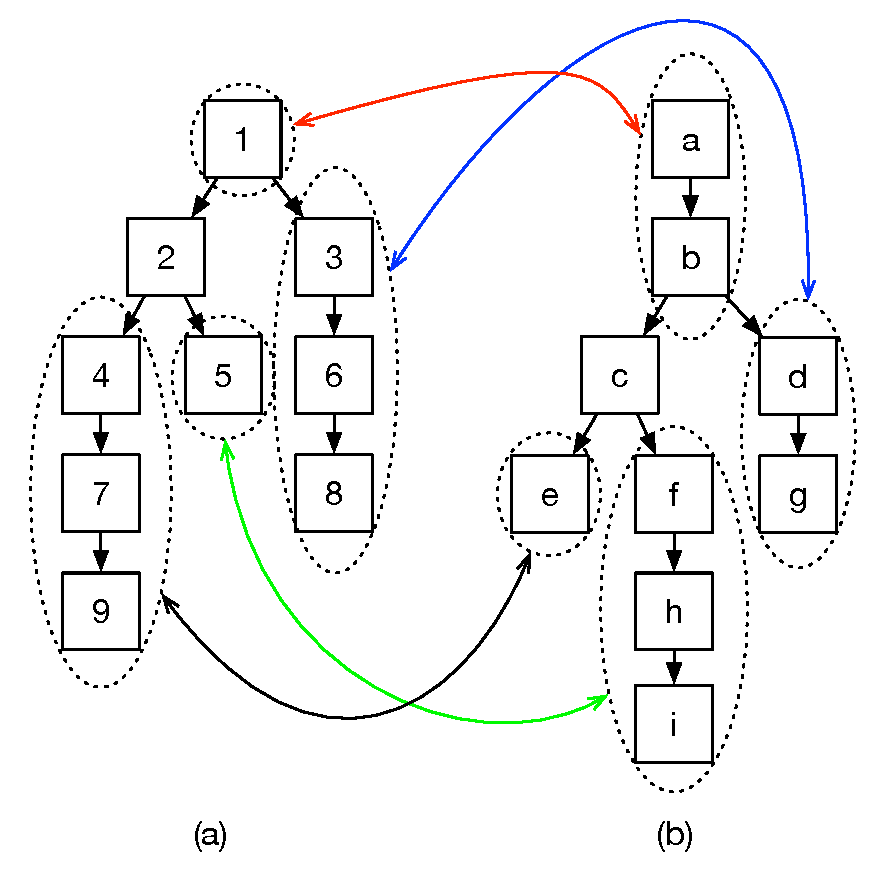
\includegraphics[width = 5cm,height=4cm]{srj-figures/srj-func_mod.pdf} %the_graph
  \caption{A sample signature (a) and target (b) functions, where the lines indicate the matched partial traces and the nodes refer to the basic-blocks.} \label{fig:func_mod}
%\vspace{-1mm}
\end{figure}


In \tool, we leverage on length variant partial traces to model the functions. %The key advantage of using partial trace over other techniques~\cite{DBLP:conf/pldi/DavidY14, DBLP:conf/sp/PewnyGGRH15,luo2014semantics,sebastian2016discovre} lies in its resilience to the structural changes. %To this end,
We generate partial traces with three different lengths (i.e., $k=1,2$ and $3$) from each function, all of which collectively constitute the function model. For example, function models generated from the signature ($\mathcal{M}_{sig}$) and target ($\mathcal{M}_{tar}$) functions in Fig.~\ref{fig:func_mod} are listed as follows:

\begin{itemize}
\small
\itemsep0em
  \item[] $\mathtt{\mathcal{M}_{sig}:  \lbrace \langle 1 \rangle,  \langle 2 \rangle,\ldots, \langle 1,2 \rangle, \langle 2,5 \rangle, \ldots, \langle 1,2,4 \rangle, \langle 2,4,7 \rangle,\ldots\rbrace}$
   \item[] $\mathtt{\mathcal{M}_{tar}: \lbrace \langle c \rangle,  \langle b \rangle, \ldots, \langle a,b \rangle, \langle b,c \rangle, \ldots, \langle a,b,c \rangle, \langle b,c,f \rangle, \ldots \rbrace}$
\end{itemize}

In \tool and \toolNew, we support the function model similarity matching in terms of \textit{n-to-m}, \textit{1-to-n}, \textit{n-to-1} and \textit{1-to-1} partial trace matching across the signature and target functions, mitigating the impact of program structural difference.
\begin{description}
\itemsep0em
  \item[\textit{n-to-m}] Partial traces of length $n (\in\mathbb Z_{> 1})$ generated from the signature function are matched against the partial traces of length $m (\in\mathbb Z_{> 1})$ generated from target function. In Fig.~\ref{fig:func_mod}, matching partial traces $\langle 3,6,8\rangle$ and $\langle d,g\rangle$ is \textit{3-to-2} matching.
  \item[\textit{1-to-n}] A basic-block (i.e., a partial trace of length 1) in the signature function is matched against the partial traces of   length $n (\in\mathbb Z_{> 1})$ generated from target function. In Fig.~\ref{fig:func_mod}, partial traces $\langle 1\rangle$ and $\langle 5\rangle$ are matched with $\langle a,b\rangle$ and $\langle f,h,i\rangle$, respectively.
  \item[\textit{n-to-1}] Partial traces of length $n (\in\mathbb Z_{> 1})$ generated from the signature function are matched against a basic-block in the target function. In Fig.~\ref{fig:func_mod}, partial trace $\langle 4,7,9 \rangle$ is matched with $\langle e \rangle$.
  \item[\textit{1-to-1}] A basic-block in the signature function is matched against a basic-block in the target function. It is also known as pairwise comparison at the level of single basic-block. In Fig.~\ref{fig:func_mod}, partial trace $\langle 2\rangle$ is matched with $\langle c\rangle$.
\end{description}

\textit{1-to-n} matching addresses the issue of basic-block splitting --- a single basic block in the signature function is split into several smaller basic blocks in the target function. Similarly, \textit{n-to-1} matching addresses the basic-block merging problem.
%On the other hand, \textit{n-to-m} mapping is generally preferred when the signature (target) function is part of a huge target (signature) function and appropriately selected values for $n$ and $m$ will maximize the function similarity. Finally, if none of the aforementioned matching techniques work, we resort to \textit{1-to-1} matching to compare the basic-block similarity in a pairwise way, which is similar to those basic-block centric comparison approaches~\cite{DBLP:conf/sp/PewnyGGRH15,luo2014semantics}.
In tracelet modeling \cite{DBLP:conf/pldi/DavidY14}, authors recommended that both the signature and target should be of the same size (i.e., $k=3$), and hence only \textit{n-to-n} matching is performed.
In~\cite{DBLP:conf/sp/PewnyGGRH15} and~\cite{luo2014semantics}, pairwise comparison of single basic-block (i.e., \textit{1-to-1} matching) is performed as an initial step to shortlist target functions. In contrast, in \tool and \toolNew, all the  4 types of function matching are needed to cover all possible BB-structure variances that arise due to architecture, OS and compiler differences.


For the similarity score of using low-level semantic features $\mathcal{SIM_{L}}(sig, tar)$, considering the function model as a bag of partial traces, Jaccard containment similarity~\cite{agrawal2010indexing} is also used to measure the similarity of two different function models:
\begin{equation}
\begin{aligned}
 \mathcal{SIM_{L}}(sig, tar)  = \frac{\mathcal{M}_{sig} \bigcap \mathcal{M}_{tar}}{\mathcal{M}_{sig}}
\end{aligned}
\end{equation}
where $\mathcal{M}_{sig}$ and $\mathcal{M}_{tar}$ refer to function models of low-level semantics that are generated from signature and target functions, respectively.

%
%Finally, considering the function model as a bag of partiral traces, Jaccard containment similarity~\cite{agrawal2010indexing} is used to measure the similarity score between  two different function models, and is defined below:
%\begin{equation}
%\begin{aligned}
% sim(\mathcal{M}_{sig}, \mathcal{M}_{tar}) = \frac{\mathcal{M}_{sig} \bigcap \mathcal{M}_{tar}}{\mathcal{M}_{sig}}
%\end{aligned}
%\end{equation}
%where $\mathcal{M}_{sig}$ and $\mathcal{M}_{tar}$ refer to function models generated from signature and target functions, respectively.

%In \tool, the function model matching is not fixed, where, for a given signature function, the searching algorithm will try all possible function models and pick the best one that maximizes the signature-target function similarity. In contrast, the techniques proposed in the literature do not have the flexibility to try out all possible matchings. For example, in tracelet-based modeling \cite{DBLP:conf/pldi/DavidY14}, the authors recommended that the tracelet size should be larger (e.g., $k>2$), for both signature and target functions, hence, only \textit{n-to-m} matching is performed, in fact, it is \textit{n-to-n} matching as they consider the same tracelet size for both signature and target functions. Further, in~\cite{DBLP:conf/sp/PewnyGGRH15} and~\cite{luo2014semantics}, pairwise comparison of basic-blocks (i.e., \textit{1-to-1} matching) is performed as an initial step to identify potential target functions, which inherently assumes that the program structure is maintained across signature and target functions and at least one basic-block in the target function resembles a basic-block in the signature function.

%\subsection{Locality Sensitive Hashing} \label{subsec:lsh} %\note{replace this with simple feature hasing technique, if no time, leave as it is.. not very important}
%In \tool, we leverage on Locality-sensitive Hashing (LSH) technique to perform the function matching more efficiently and in a scalable manner. Locality-sensitive hashing is an algorithm for searching similar items in large and high dimensional dataset \cite{leskovec2014mining} based on the assumption that, if two items are similar, the hashed value of the two items will remain similar. In \tool, we use MinHashing~\cite{broder1997resemblance} technique to hash the extracted features and generate hash signature for each function model. To this end, we use 1000 (i.e., $n=1000$) hash functions to generate the signature, which leads to an error of 3.16\%. The similarity between two function model is given by this equation:
%\begin{equation}
%\begin{aligned}
% sim(mh_a, mh_b) = \frac{\vert mh_a[i]=mh_b[i ]\vert}{n}
%\end{aligned}
%\end{equation}
%where the jaccard similarity between two function models is approximated by MinHash similarity between the two models.

%\subsubsection{Function Model Generation} \label{subsec:fun_mod_mat}

%\subsection{Primary Matching and Final Matching} \label{subsec:sem_fea_ext}
%\subsubsection{Primary Matching}
\subsection{Final Matching} \label{subsec:matching:final}

To remove false positives of using low-level semantics alone, $\mathcal{SIM^\prime}(sig, tar)$ is also considered in the final matching.

Let $\mathcal{SIM^*}(sig, tar)$ denote the overall similarity score calculated in the final matching. $\mathcal{SIM^*}(sig, tar)$ is calculated as the weighted sum of $\mathcal{SIM^\prime}(sig, tar)$ and  $\mathcal{SIM_{L}}(sig, tar)$. Here, we adopt two strategies for different matching scenarios.

If the matching is based on the same code base, we consider both $\mathcal{SIM_{L}}(sig, tar)$ and $\mathcal{SIM^\prime}(sig, tar)$ are equally important.
\begin{equation}
\begin{aligned}
 \mathcal{SIM^*}(sig, tar) =  (1/2) * \mathcal{SIM^\prime}(sig, tar)  \\
  + (1/2) * \mathcal{SIM_{L}}(sig, tar)
\end{aligned}
\end{equation}


Otherwise, if the matching is based on different code bases (i.e., experiments on cross-OS matching), we ignore the structural features and give equal weight for low-level semantics and high-level semantics.
\begin{equation}
\begin{aligned}
 \mathcal{SIM^*}(sig, tar) =  (1/2) * \mathcal{SIM_H}(sig, tar)  \\
  + (1/2) * \mathcal{SIM_{L}}(sig, tar)
\end{aligned}
\end{equation}

\xyx{Still take the code segments in Fig.~\ref{fig:falseposi} as example. The two code segments are from different code bases, and hence the BB structure will not be similar. Low-level semantics and high-level semantics are used together to measure their semantic similarity. Previously,  in \tool, using low-level semantics alone suggests they have a similarly value of 0.7 --- 70\% of tracelets in the signature function match the target function on I/O value pairs. Now, in \toolNew, since they have a low high-level similarity of 0.7 and no similarity in high-level features and structural features, their overall similarity is lower to 0.35. Hence, the false positive has a lower similarity score, and will be removed from the best-match or top-5-match list.}
